
\subsection{Редактор sc.g-текстов}

Текущая реализация редактора sc.g-текстов работает с SCg-кодом версии 0.1.0.

Описываемый в данном разделе редактор sc.g-текстов, работает с sc.g-текстами записанными с помощью SCg-кода версии 0.1.0.


При редактировании некоторого фрагмента, с помощью SCg-кода, доступны следующие типы sc.g-элементов: {\sf sc.g-узел}, {\sf sc.g-дуга}, {\sf sc.g-шина}, {\sf sc.g-контур}.
 
Чтобы упростить процесс редактирования sc.g-конструкций выделены различные режимы редактирования. В каждом из таких режимов редактирования пользователь может создавать объекты определенноги вида. Основыне режимы редактирования и часть команд вынесены на панель инструментов. 
\begin{figure}[h]
	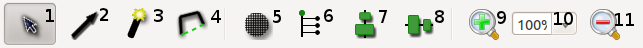
\includegraphics[width=15.77cm, height=1.27cm]{../images/scgtoolbar.png}
	\caption{Панель инструментов: 1 – режим выделения; 2 – режим создания дуг; 3 – режим создания шин; 4 – режим создания контуров; 5 – выравнивание по сетке; 6 — выравниваение связки с шиной; 
7 – выравнивание по вертикали; 8 – выравнивание по горизонтали; 9 – увеличение масштаба; 10 – установка значения масштаба графической сцены; 11 – уменьшение масштаба.}
	\label{scgtoolbar}
\end{figure}

Рассмотрим имеющиеся режимы редактирования и команды, которые вынесены на панель инструментов:
\begin{enumerate}
	\item Режим \textbf{выделения и перемещения объектов}. В данном режиме пользователь может работать со всеми объектами выделяя их, перемещая их, вызывая контекстное меню с командами. 
Отличительной особенностью данного режима является то, что в нем можно создавать {\sf sc.g-узлы}. Для этого необходимо выполнить двойной клик мышью в месте, где необходимо создать узел (в момент создания под указателем мыши не должно быть других объектов);
	\item Режим \textbf{создания дуг}. Создание дуги начинается с того, что пользователь указывает объект из которого она быдет выходить (клик левой клавиши мыши), далее он может указать точки излома дуги (клик левой клавиши мыши, в пустом месте документа), завершается создание указанием конечного объекта (клик левой клавиши мыши). В процессе создания пользователь может отменять последнее действие (указание начального объекта, точки излома) путем клика правой клавиши мыши;
	\item Режим \textbf{создания шин}. Шины используются для увелечения контактной площади узла, поэтому они могут создаваться лишь для узлов. Создание шины начинается с указания узла, для которой она создается (клик левой клавиши мыши), далее как и при создании дуг указываются точки излома. Завершается создание шины путем клика на последней точке излома (при наведении на нее, рисуется {\bf\it сплошная линия}). Как и при создании дуг пользователь может отменять последнее действие нажатием правой клавиши мыши;
	\item Ррежим \textbf{создания контуров}. Создание контура заключается в указании его точек. Завершается процесс кликом левой клавиши мыши на начальной точке (при наведении на нее появляется сплошная линия).  Как и при создании дуг и шин пользователь может отменять последнее действие нажатием правой клавиши мыши;
	\item Команда \textbf{выравнивания объектов по сетке}. Данная команда позволяет выровнять объекты имеющиеся в документе по сетке. Размеры сетки указываются при инициировании команды в диалоге настроек.
\begin{figure}[h]
	\centering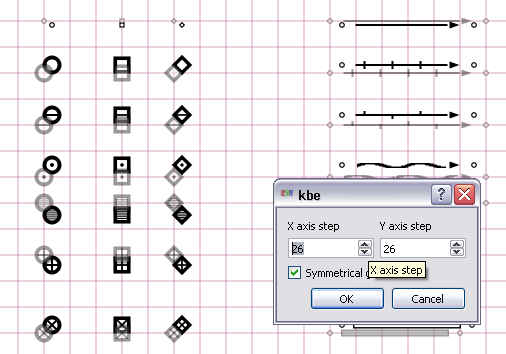
\includegraphics[height=10.98, height=5.75cm]{../images/gridaligment.png}
	\caption{Пример использования команды выравнивания по сетке}
	\label{gridaligment}
\end{figure}
В диалоговом окне, которое появляется после инициирования команды, можно установить желаемые размеры сетки (см. Рисунок~\ref{gridaligment}).
	\item Команда \textbf{выравнивания связки с шиной}. Данная команда позволяет выровнять узел у которого имеется шина, с выходящими (выходящими) дугами. Как и в случае выравнивания по сетке, при инифиировании команды появляется окно настроек (см. Рисунок~\ref{tuplealigment}). Для инициирования команды необходимо выделить узел из которого выходит шина.
	
\begin{figure}[h]
	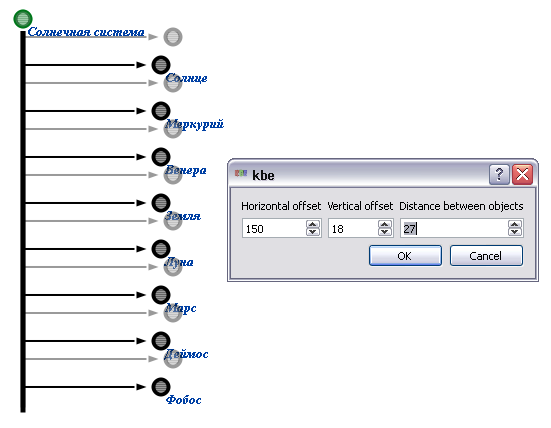
\includegraphics[width=13.07cm, height=9.82cm]{../images/tuplealigment.png}
	\caption{Пример использования команды выравнивания связки с шиной}
	\label{tuplealigment}
\end{figure}
	\item Команда \textbf{выравнивания по вертикальной линии}. Инициирование команды приводит к выравниванию по X координате выделенных объектов. Новая координата считается как среднее арифметическое X координат выделенных объектов. Y координаты объектов не меняются. Команда не имеет настроек;
	\item Команда \textbf{выравнивания по горизонтальной линии}. Инициирование команды приводит к вырваниванию по Y координате выделенных объектов. Новая координата считается как среднее ариaметическое Y координат выделенных объектов. X координаты объектов не меняются. Команда не имеет настроек;
	\item Команда \textbf{увеличения масштаба}. Инициирование команды приводит к увеличению масштаба изображения;
	\item Список \textbf{стандартных масштабов}. Элемент управления, который позволяет выбрать масштаб из уже заранее имеющихся, либо указать свой масштаб;
	\item Команда \textbf{уменьшения масштаба}. Инициирование команды приводит к уменьшению масштаба изображения.
\end{enumerate}

\hrule
\smallskip
\noindent
\includegraphics[width=25pt, height=25pt]{../images/note.png} \textcolor[rgb]{.67,.05,.05}{Каждый режим можно инициировать нажатием клавиш 1-4. Также и команды выравнивания клавишами 5-8.}
\smallskip
\hrule
\smallskip
\hrule
\smallskip
\noindent
\includegraphics[width=25pt, height=25pt]{../images/note.png} \textcolor[rgb]{.67,.05,.05}{Рекомендуем использовать выравнивание по сетке и связок с шиной. Настроив единажды размеры сетки или параметры для шины, вы можете используя горячие клавиши 5 и 6 быстро ровнять конструкции.}
\smallskip
\hrule
\medskip
Кроме перечиленных выше команд существует еще целый ряд команд редактирования:
\begin{itemize}
	\item Команда \textbf{изменения основного текстового идентификатора элемента}. Любому sc.g-элементу можно устанавливать некоторый текстовый идентификатор. Для того, чтобы установить (изменить) текстовый идентификатор sc.g-элемента, необходимо в контекстном меню данного элемента выбрать пункт “\textbf{Изменить идентификатор}”, либо воспользоваться \textit{горячей клавишей} \textbf{I}. После чего будет вызвано диалоговое окно, в котором вы сможете ввести необходимый идентификатор (см. Рисунок~\ref{idtfdialog}).
	\begin{figure}[h]
		\centering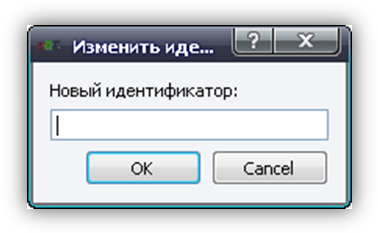
\includegraphics[width=6.70cm, height=3.92cm]{../images/idtfdialog.png}
		\caption{Диалоговое окно изменения текстового идентификатора}
		\label{idtfdialog}
	\end{figure}
	\item Команда \textbf{изменения типа элемента}. Позволяет изменять тип sc.g-элемента (константность, структурный тип и т.д.). Доступные типы можно открыть нажатием правой клавиши мыши на элементе (тип которого будет изменяться) и выборе нужного типа в меню \textbf{Изменить тип};
	\item Команда \textbf{установки содержимого}. Установить содержимое для sc.g-узла достаточно просто, для этого необходимо  нажать правой клавишей мыши на узле и выбрать команду установки содержимого. После инициирования команды появляется диалог, в котором можно выбрать тип содержимого и само содержимое (см. Рисунок~\ref{contentdialog})
	\begin{figure}[h]
		\centering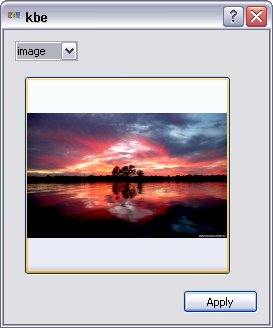
\includegraphics[width=6.09cm, height=7.46cm]{../images/contentdialog.png}
		\caption{Диалог установки содержимого}
		\label{contentdialog}
	\end{figure}
	\hrule
\smallskip
\noindent
\includegraphics[width=25pt, height=25pt]{../images/lamp.png} \textcolor[rgb]{.25, .67, .2}{\textbf{Примечание}: Есть альтернативный и более простой способ установки содержимого из файла. Для этого надо лишь перетянуть файл на окно, после чего создастся sc.g-узел в содержимом которого будет установлен перетаскиваемый файл.}
\smallskip
\hrule
\end{itemize}
